\documentclass[12pt]{article}
\usepackage{setspace}
\usepackage{graphicx}
\usepackage{amsmath}
\RequirePackage[colorlinks]{hyperref}

\setstretch {1.25} 
\usepackage{geometry}
\geometry{papersize={21cm,29.7cm}}
\geometry{left=2.5cm,right=2.5cm,top=3cm,bottom=3cm}
\usepackage{fancyhdr}
\usepackage{listings}
\usepackage{color}
\usepackage{gensymb}
%\usepackage{showframe}

\usepackage[normalem]{ulem}
\definecolor{mygreen}{RGB}{28,172,0} % color values Red, Green, Blue
\definecolor{mylilas}{RGB}{170,55,241}
\definecolor{black}{rgb}{0,0,0}
\definecolor{olivegreen}{RGB}{112,161,71}
\definecolor{lakeblue}{RGB}{0,127,255}
\definecolor{orange}{RGB}{255,139,0}
\definecolor{purple}{RGB}{102,0,255}
\pagestyle{fancy}
\lhead{\author}
\chead{\date}
\lfoot{}
\cfoot{\thepage}
\rfoot{}
\renewcommand{\headrulewidth}{0.4pt}
\renewcommand{\headwidth}{\textwidth}
\renewcommand{\footrulewidth}{0pt}
\newcommand{\alert}[1]{{ \color{purple} [{#1} ]}}

\newcommand{\vect}[1]{\mathbf{#1}}

\DeclareMathOperator*{\argmin}{arg\,min}
\DeclareMathOperator*{\argmax}{arg\,max}


\title{Research Notes}
%\author{KEG}
%\date{\today}
\begin{document}
	\maketitle
	\lstset{language=Matlab,%
	    %basicstyle=\color{red},
	    breaklines=true,%
	    morekeywords={matlab2tikz},
	    keywordstyle=\color{blue},%
	    morekeywords=[2]{1}, keywordstyle=[2]{\color{black}},
	    identifierstyle=\color{black},%
	    stringstyle=\color{mylilas},
	    commentstyle=\color{mygreen},%
	    showstringspaces=false,%without this there will be a symbol in the places where there is a space
	    numbers=left,%
	    numberstyle={\tiny \color{black}},% size of the numbers
	    numbersep=9pt, % this defines how far the numbers are from the text
	    emph=[1]{for,end,break},emphstyle=[1]\color{red}, %some words to emphasise
	    %emph=[2]{word1,word2}, emphstyle=[2]{style},    
	}
	

\section{Introduction}
\subsection{Background}

Ebola virus disease (EVD) is a lethal human and primate disease that currently requires a particular attention from the international health authorities due to important outbreaks in some Western African countries and possible spread to other continents, in fact, it has already occurred in west countries such as the USA , UK and Spain. Regarding the emergency of this situation, there is a need of development of decision tools to assist the authorities to focus their efforts in important factors to eradicate Ebola.

In particular, mathematical modelling can help to predict the possible evolution of the Ebola outbreaks and to give some recommendations about how to control the situation.

In this work, we propose a novel spatial and temporal model based on TBD, called TBD, to study the evolution of EVD in Sierra leone, Liberia and Guinea, which has owned the most serious situations due to their poor health care system. We use the city as the basic research object to simulate the spread of Ebola disease and identify risk zones. The main interesting Characteristics of TBD are the consideration of the migratory flux between cities and control measure effects and the use of time dependent evolution adapted to each city.

First, we focus on the mathematical formulation of each component of the model. Next, in order to validate our approach, we consider various numerical experiments regarding the 2014 Ebola epidemic. In particular, we study the ability of the model in predicting the EVD until the end of the epidemic.

The results are compared to real data and other models outputs found in the literature. Finally, a brief parameter sensitivity analysis is done.

\subsection{Problem Restatement}

The world medical association has announced that their new medication could stop Ebola and cure patients whose disease is not advanced. Build a realistic, sensible, and useful model that considers not only the spread of the disease, the quantity of the medicine needed, possible feasible delivery systems (sending the medicine to where it is needed), (geographical) locations of delivery, speed of manufacturing of the vaccine or drug, but also any other critical factors your team considers necessary as part of the model to optimize the eradication of Ebola, or at least its current strain. In addition to your modeling approach for the contest, prepare a 1-2 page non-technical letter for the world medical association to use in their announcement.

The goal of this project's core is to control the disease outbreak, on the basis of the goal, assume that the drug has a certain production capacity, we focus on delivery the drug to the city which is most needed.


\subsection{Assumptions}

Based on the background of the Ebola virus, the spread of disease only consider the interpersonal communication. So we only focus on the population flow effect on the spread of the disease. We have established a network based on geographical location, the spread of the disease is considered as the network segment.

\begin{itemize}

\item	Lattice point in the network on behalf of each city, there are two directed line segment between different cities, represents the spread of disease is a two-way flow
\item	The population of each city is already known
\item	Infections caused by migration between cities, the population flow between cities is positive correlation with their population, and negative correlation with the distance between them. City whether belong to the same countries or not also affects the population movement.
\item	In our work, we don’t consider the virus variation. At the same time, We don't intend to distinguish different Ebola virus subtype.



\end{itemize}
\section{Cascaded Poisson Process}
Multi-dimensional Hawkes process\cite{zhou2013learning} are used to model repeated events and influence between people. It provided inspiration for us to model the infections of disease as a inhomogeneous Poisson Process to track the temporal and spatial behaviour of disease transmissions.

From Fig.~\ref{new} we can see the new infections, we model the new infections as a diffusion process. We consider the diffusion process using discrete time steps.

One person being infected is a point process, so viewing it from a higher level, the infection is a Poisson Process.

The intensity of the Poisson Process is related to many factors. 

The intensity in one city/area depends on two parts, one part comes from itself, and the second part comes from all other cities. 


$$\sigma_{i,j} = \frac{Po_i^{\beta_1}Po_j^{\beta_2}}{d_{i,j}^{\beta_3}}$$


For simplification, we set:

$$\beta_1 = 1, \beta_2 = 1, \beta_3 = 2$$

TBD cite:gravity model

$\sigma$ is defined as the distance between two cities, and the distance from a city to itself is the unit distance. 

$$\mu_{i,t_k} = \lambda_1 \sum_{m = 1}^{ k-1} P_{i,t_m} e^{-\beta(k-1-t)} + \lambda_2 \sum_{j:j\neq i} \sum_{m = 1}^{ k-1} P_{j,t_m} \sigma_{j,i} e^{-\beta(k-1-t)}$$

We do a MLE to fit the data to the model and get $\lambda_1$ and $\lambda_2$.

The likelihood function is:

$$L(\lambda_1, \lambda_2) = \prod_{i \in V} \prod_{k} \frac{(\mu_{i,t_k}\Delta t)^{P_{i,t_k}} e^{-\mu_{i,t_k}\Delta t}}{P_{i,t_k}!}
$$


$$
\log L(\lambda_1, \lambda_2) = \sum_{i \in V} \sum_{k}\left[ {P_{i,t_k} \log{(\mu_{i,t_k}\Delta t)} {-\mu_{i,t_k}\Delta t}} - \log{P_{i,t_k}!} \right]
$$


$$
\frac{\partial \log L(\lambda_1, \lambda_2)}{\partial \lambda_1} = \sum_{i \in V} \sum_{k}\left[ {P_{i,t_k} \frac{ \frac{\partial \mu_{i,t_k}}{\partial \lambda_1}}{\mu_{i,t_k}} {- \frac{\partial \mu_{i,t_k}}{\partial \lambda_1}\Delta t}} \right] 
$$


$$
\frac{\partial \log L(\lambda_1, \lambda_2)}{\partial \lambda_2} = \sum_{i \in V} \sum_{k}\left[ {P_{i,t_k} \frac{ \frac{\partial \mu_{i,t_k}}{\partial \lambda_2}}{\mu_{i,t_k}} {- \frac{\partial \mu_{i,t_k}}{\partial \lambda_2}\Delta t}} \right] 
$$

Solve for equation 1:

$$
\frac{\partial \log L(\lambda_1, \lambda_2)}{\partial \lambda_1} = \sum_{i \in V} \sum_{k}\left[ { \frac{P_{i,t_k}\sum_{m = 1}^{ k-1} P_{i,t_m} e^{-\beta(k-1-t)}}{ \lambda_1 \sum_{m = 1}^{ k-1} P_{i,t_m} e^{-\beta(k-1-t)} + \lambda_2 \sum_{j:j\neq i} \sum_{m = 1}^{ k-1} P_{j,t_m} \sigma_{j,i} e^{-\beta(k-1-t)}}} \right.
$$
$$
\left. {- \left( \sum_{m = 1}^{ k-1} P_{i,t_m} e^{-\beta(k-1-t)} \right)\Delta t} \right] 
$$

solve for equation 2:

$$
\frac{\partial \log L(\lambda_1, \lambda_2)}{\partial \lambda_2} = \sum_{i \in V} \sum_{k}\left[ { \frac{P_{i,t_k}\sum_{j:j\neq i} \sum_{m = 1}^{ k-1} P_{j,t_m} \sigma_{j,i} e^{-\beta(k-1-t)} }{ \lambda_1 \sum_{m = 1}^{ k-1} P_{i,t_m} e^{-\beta(k-1-t)} + \lambda_2 \sum_{j:j\neq i} \sum_{m = 1}^{ k-1} P_{j,t_m} \sigma_{j,i} e^{-\beta(k-1-t)}}} \right.
$$
$$
\left. {- \left( \sum_{j:j\neq i} \sum_{m = 1}^{ k-1} P_{j,t_m} \sigma_{j,i} e^{-\beta(k-1-t)} \right)\Delta t} \right] 
$$

All the terms are positive. So use gradient descent to find the solution.

$$\lambda_1^* = \lambda_1 - \gamma \frac{\partial \log L(\lambda_1, \lambda_2)}{\partial \lambda_1}$$

$$\lambda_2^* = \lambda_2 - \gamma \frac{\partial \log L(\lambda_1, \lambda_2)}{\partial \lambda_2}$$

$\gamma$ is the step size.





\section{Plots}


\begin{figure}[hbt]
\begin{center}
  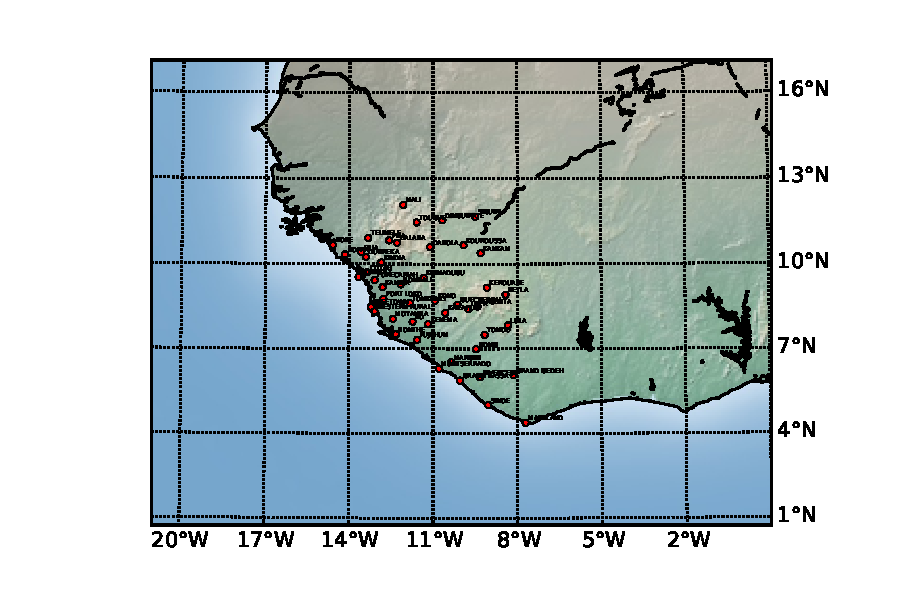
\includegraphics[width=6in]{graph/map2.pdf}
  \caption{Location of Ebola infected cities}
\end{center}  
\end{figure}

\begin{figure}[hbt]
\begin{center}
  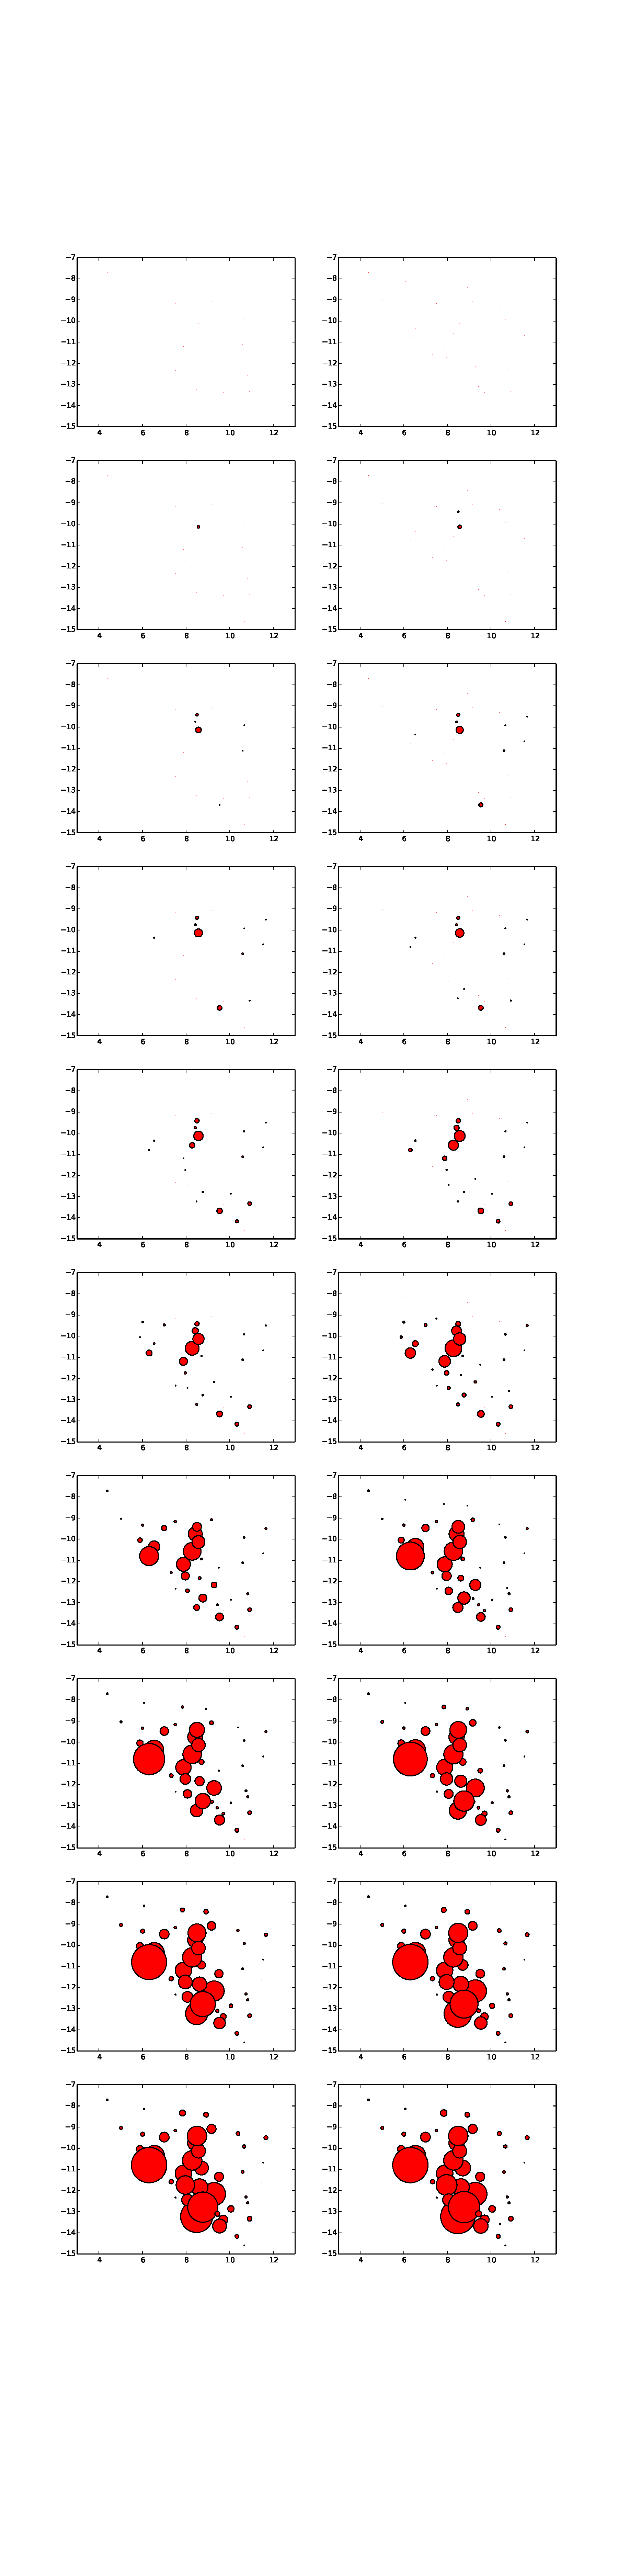
\includegraphics[width=2in]{graph/evlvo.pdf}
  \caption{Progress of Ebola outbreak}
\end{center}  
\end{figure}

\begin{figure}[hbt]
\begin{center}
  
\includegraphics[width=2in]{graph/new2.pdf}
  \caption{New infections of Ebola outbreak}
  \label{new}
\end{center}  
\end{figure}


\begin{figure}[hbt]
\begin{center}
  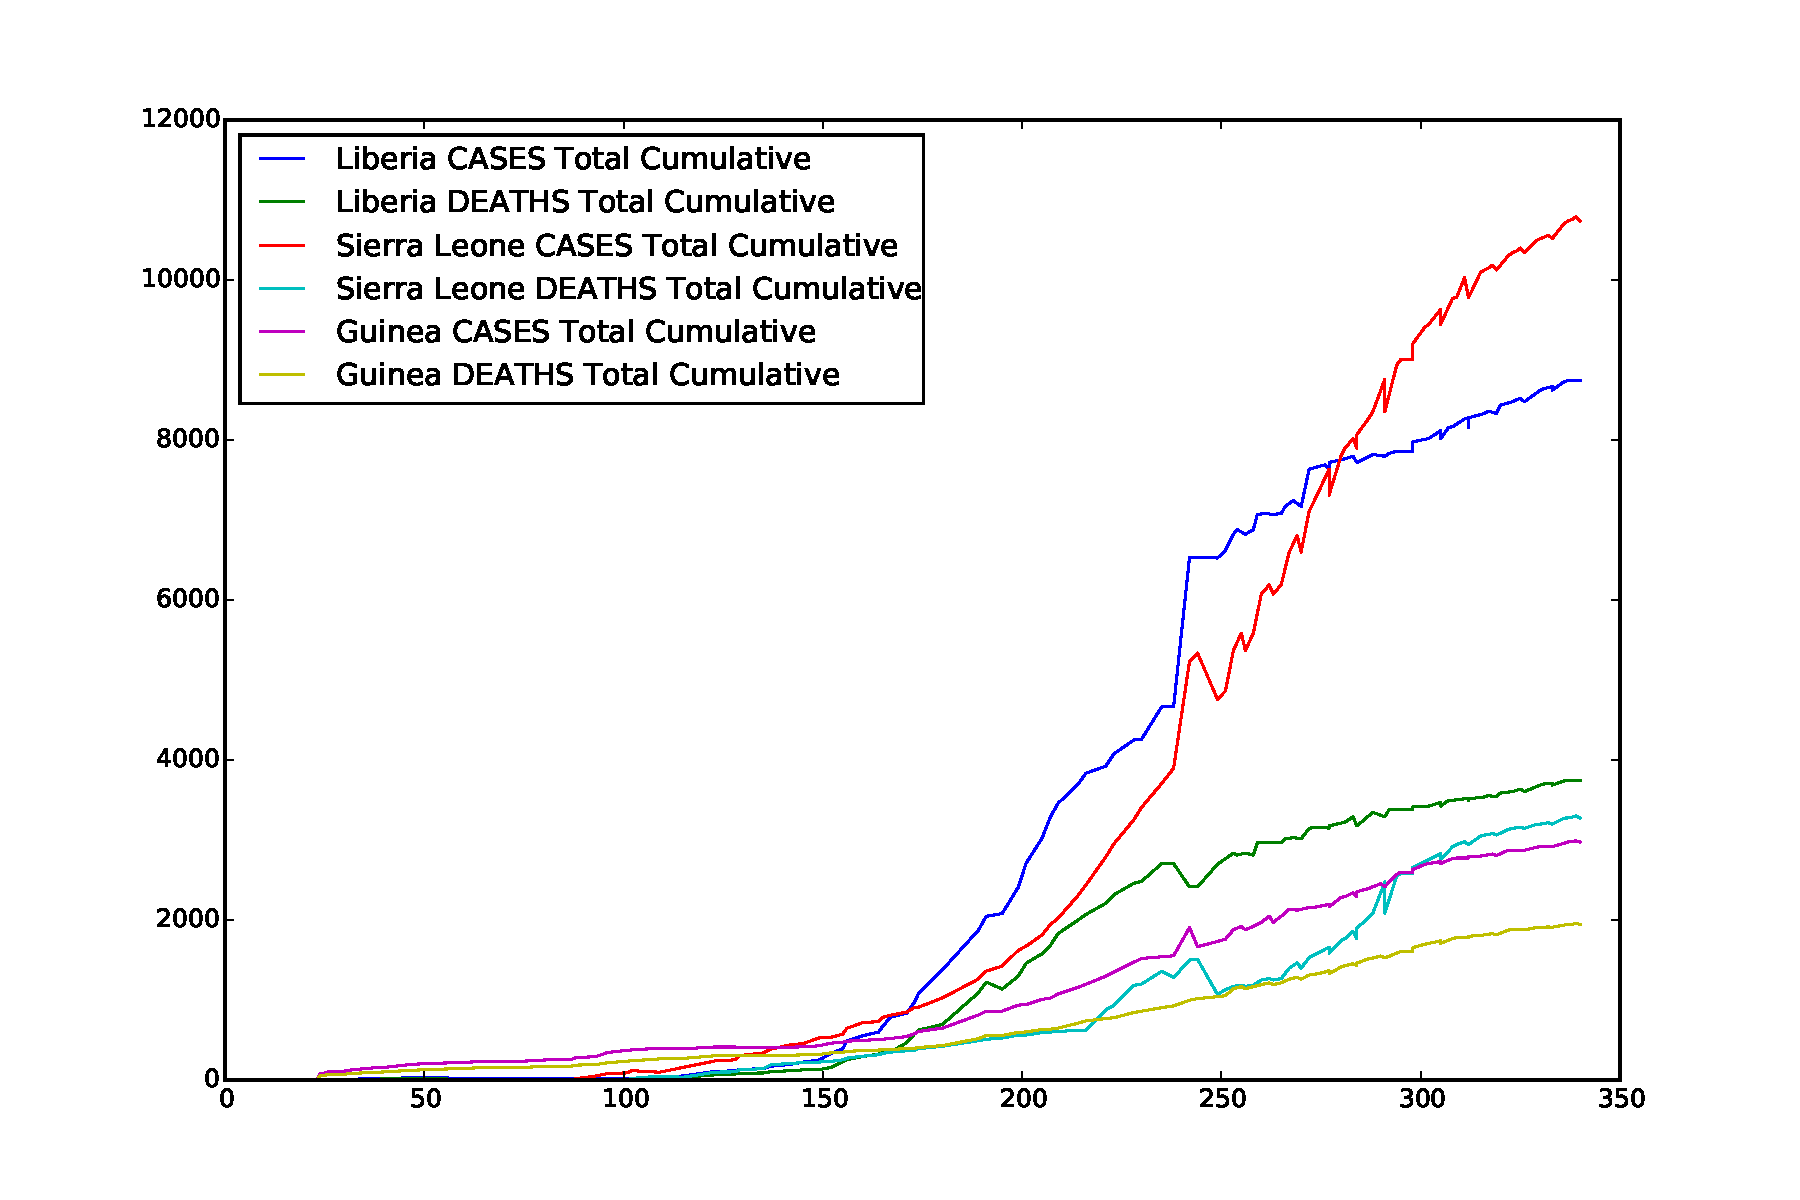
\includegraphics[width=6in]{graph/stats.pdf}
  \caption{General statistics of Ebola outbreak}
\end{center}  
\end{figure}

\bibliography{ref}
\bibliographystyle{ieeetr}
\end{document}